\chapter{Methods}

We describe how we made the tool proposed in this thesis. We start with a general overview
of the architecture and then zoom in on all the technical design decisions made during the implementation.

\section{Requirements}

The following prime requirements are identified to guide the implementation process.

\begin{itemize}
  \item \textbf{GHC $\geq$ 8.4 cross compatible} - Important to facilitate inspecting the effects of changes in the compiler on the same source.
  \item \textbf{Simple and non invase steps to create dumps} - Large and established code bases should be able to use the tool.
  \item \textbf{Cross-platform ability to explore dumps} - The tool should be able to run on all major platforms, preferably without any additional dependencies.
  \item \textbf{Extendable} Not everything needs to be supported (think unfoldings) but should be extendable in the future.
\end{itemize}

\section{Architecture}

We envisioned a high degree of interactability with the snapshots of the intermediate ASTs. To realise this
in a cross-platform, dependency-free, fashion, we decided to use a browser based frontend application. 
Because the concept of mutually recursive algebraic datatypes are very pervasive in the Core AST, we felt it would be 
extremely helpful if the frontend language had first class support for this. This quite naturally led to us to Elm, a functional language
that compiles to Javascript \cite{elm_lang}.

\begin{figure}[h]
  \centering
  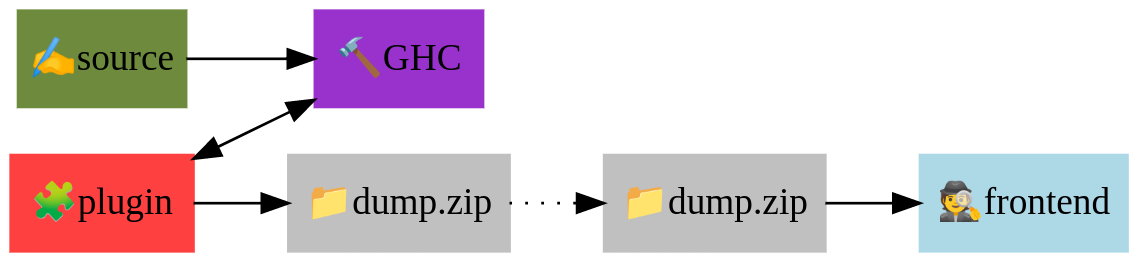
\includegraphics[width=0.8\textwidth]{figs/architecture.png}
  \caption{Dataflow diagram of the tool}
  \label{fig:architecture}
\end{figure}


% \digraph{abc}{
%   rankdir=LR
%     
%   source [label = "✍source",shape=MSquare, color="darkolivegreen4",style=filled]
% 
%   subgraph plugin {
%     style=filled;
%     color=lightgrey;
%     node [style=filled,color=gray,shape=box];
%     label = "plugin";
%     
%     ghc [label="🔨GHC",color="darkorchid"]
%     plugin [color="brown1",label="🧩plugin"]
%     dump1 [label = "📁dump.zip"]
%     dump2 [label = "📁dumb.zip"]
%   
%     source -> ghc
%     plugin -> ghc [dir=both]
%     plugin -> dump1
%     dump1 -> dump2 [style=dotted]
%   
%     dump2 -> frontend
%   }
% 
%   subgraph frontend {
%     node [style=filled];
%     label = "frontend";
%     color=blue
%     frontend [color=lightblue,label="🕵frontend"]
%   }
% }
% 
\section{Creating the GHC plugin}

The least invasive option would be to parse the output of GHC given a number of \mono{-ddump} flags. However, for the sake
of convenience and robustness, we instead decided to create a plugin that hook directly into the core2core pipeline and
capture the ASTs completely has original value. By interspersing each transformation with snapshot action we have complete information
and freedom. 

\subsection{Capturing the information}
\label{section:methods:capturing_info}

If we wish to support multiple recent versions of GHC we need to deal with the fact that the Core ADT has undergone
a few minor changes and additions. We believe that the solution is to create some auxiliary definition to which we can
map various versions of the Core ADT. This was done very efficiently by building upon the existing \mono{ghc-dump} package,
which already implemented such a representation as well as a version agnostic conversion module with the help of \mono{min_version_GHC}
macro statements \cite{ghc_dump}. 

What \mono{ghc-dump} also intelligently addresses, is the issue of possible infinite recursion.
This problem arises through the \mono{IdInfo} struct attached to each variable such that the inliner
knows the body of variable when it wishes to inline the variable. However, when a variable represents a recursive ---
or even mutually recursive --- value, the inlining will contain itself. This fact implies that we can never serialise 
the AST to a finite value. Therefore, \mono{ghc-dump} demotes each usage site of a variable to an identifier referencing its binding site.
This allows us to obtaining a finite representation that we can later reconstruct by traversing
the AST with an environment.

\subsection{Globally unique variables}

It is not strictly necessary for variable names in a program to be unique. A variable name always
references the nearest binding site; So too in Core. However, is not very convenient
when we want to analyze a certain variable in isolation. After all, we cannot know if two separate free variables
with the same name are actually the same variable or live in a different scope. Consider the definition of tail:

\begin{listing}[H]
\begin{minted}[linenos]{haskell}
tail xs = case xs of
  x:xs -> xs
  _    -> error "tail of empty list"
\end{minted}
\end{listing}

We cannot simply refer to the variable \mono{xs} as that name has two different binding sites.
We solve this by running a \textit{uniquefication} as part of each snapshot that freshens all duplicate names in the entire
module after each core2core transformation. This gives us the ability to refer to a binding site and its usages unambiguously using simply an integer.
The big idea here is that any viewing logic is completely decoupled from binding semantics:

\begin{listing}[H]
\begin{minted}[linenos]{haskell}
tail xs_0 = case xs_0 of
  x_1:xs_2 -> xs_2
  _        -> error "tail of empty list"
\end{minted}
\end{listing}

It is possible to omit the numbered suffixes when displaying the AST, but internally it is very useful to be able to make
this distinction without any further effort.

\subsection{Detecting changes}

If a module is of a slightly larger size, it becomes difficult to spot the changes made by a certain
transformation, if there even are any. To address this, we decided to develop a feature that allows for
the filtering of code that remains unchanged. Let us define what unchanged means in this context. It is
important to make the subtle distinction between syntactic equivalence and $\alpha$-equivalence. The difference
is that the latter is agnostic to the names of variables, as long as they refer to the same binding site.

We can quickly solve the decision problem of syntactic equality by calculating a hash of an expression beforehand
and simply checking for equality of this hash value. We considered using recent improvements of full sub expression
matching \cite{hashing_mod_alpha}, but decided against it as it was not clear how to effectively present the results
nor did it rarely prove useful to isolate changes in the AST as they were rarely local to begin with.
Instead, we opted for a far simpler approach where we only hash the top-level definitions, and provide a more crude
option to hide any top-level definitions that have not changed at all.

All in all, we still recommend that issues are attempted to be reproduced in small modules as the amount of
noise can quickly become overwhelming despite change detection.

\section{Creating the frontend application}

We begin with a brief introduction to the Elm language and its concepts. Very much a domain specific language, Elm is 
similar enough to Haskell to be familiar yet sufficiently simplified to be a frontend only language. The big idea is
to have \textit{pure} and \textit{complete} functions for converting the application state to html as well as handling
updates. These updates are triggered by so-called ``messages'' that are the result of user interaction. The simplicity
focused design of the language is very much affirmed by number increment/decrement example \cite{elm_lang}:

\begin{listing}[H]
\begin{minted}[linenos]{elm}
import Browser
import Html exposing (Html, button, div, text)
import Html.Events exposing (onClick)

main =
  Browser.sandbox { init = 0, update = update, view = view }

type Msg = Increment | Decrement

update msg model =
  case msg of
    Increment ->
      model + 1

    Decrement ->
      model - 1

view model =
  div []
    [ button [ onClick Decrement ] [ text "-" ]
    , div [] [ text (String.fromInt model) ]
    , button [ onClick Increment ] [ text "+" ]
    ]
\end{minted}
\end{listing}

Unlike Haskell, the lack of explicit IO means that it feels justified to disallow any form of errors and by extent incomplete functions.
This powerful property gives us great confidence in the correctness of our application.

\subsection{Reproducing the AST}

It would have been extremely tedious to have to constantly maintain a Core ADT in Elm along with a JSON
parser that is compatible with the JSON output of the Haskell plugin. Luckily, we were able to use the
\mono{haskell-to-elm} \cite{haskell_to_elm} package to automatically derive all the required boilerplate code.

For example the \mono{Alt} datatype (i.e. an arm of a case expression) is defined as follows in our AST:

\begin{listing}[H]
\begin{minted}[linenos]{haskell}
data Alt = Alt
    { altCon :: AltCon
    , altBinders :: [Binder]
    , altRHS :: Expr
    }
    deriving (Generic)

deriving instance SOP.Generic Alt
deriving instance SOP.HasDatatypeInfo Alt
type AltElm = ElmType "Generated.Types.Alt" Alt
deriving via AltElm instance Aeson.ToJSON Alt
deriving via AltElm instance HasElmType Alt
deriving via AltElm instance HasElmDecoder Aeson.Value Alt
\end{minted}
\end{listing}

Note how we derive the \mono{Aeson.ToJSON} instance via the \mono{ElmType} machinery. This control allows
us to generate a compatible and robust JSON parser for Elm. The auto-generated Elm datatype and parser
(decoder in Elm speak) look like this:

\begin{listing}[H]
\begin{minted}[linenos]{elm}
type alias Alt =
    { altCon : AltCon
    , altBinders : List Binder
    , altRHS : Expr
    }

altDecoder : Json.Decode.Decoder Alt
altDecoder =
    Json.Decode.succeed Alt |>
    Json.Decode.Pipeline.required "altCon" altConDecoder |>
    Json.Decode.Pipeline.required "altBinders" (Json.Decode.list binderDecoder) |>
    Json.Decode.Pipeline.required "altRHS" exprDecoder
\end{minted}
\end{listing}

Conveniently, it would be very easy in the future to extend the Haskell ADT with additional information
because it is the single source of truth; The Elm type and JSON machinery can then be regenerated with a single command.

Additionally, we use this pipeline embellish the AST to allow for reconstruction of the demoted call sites (see \cref{section:methods:capturing_info}).
Specifically, we add a field to each \mono{BinderId} of the type:

\begin{listing}[H]
\begin{minted}[linenos]{haskell}
type BinderThunk = Found Binder | NotFound | Untouched
\end{minted}
\end{listing}

Initially this field is set to the \mono{Untouched} variant. Once the finitely encoded AST is decoded into the 
Elm universe, a reconstruction traversal takes place that, with the help of an environment, strengthens the 
\mono{BinderThunk} with a reference to its binder. The \mono{NotFound} variant exits purely for verification purposes
and should never occur with sound inputs. It is also important to note that Elm's single static assignment
semantics naturally implies that the \mono{Binder} is never copied, but only referenced.

After this initial reconstruct we again no longer need to keep binding semantics in mind, and we can isolate
subexpressions without explicit environments.

\subsection{Pretty printing}

It certainly should be considered useful to display the Core in exactly the same way that
GHC does. After all, this is what programmers are currently already used to and its design
has been given a lot of thought. However, we felt a need to first create a separate representation
that is tailored to those who have not seen Core before.

Haskell programmers that care enough to inspect the interaction with the compiler are likely to be
avid readers of at least basic Haskell syntax. Therefore, we decided to create a pretty printer that attempts
to be as similar to Haskell source as possible. Just like GHC, we used pretty printing the method developed 
by Wadler \cite{prettier_printer}, implemented in Elm using \mono{elm-pretty-printer} \cite{prettier_printer_elm}.
We believe that such a representation is a suitable way to minimize the shock reactions in newcomers, as well as
provide a more comfortable viewing experience for those who are primarily interested in the structure of their program
throughout optimisation.

To compare, consider again the Core representation presented in \cref{section:background:ghc} with the quicksort
representation produced by our pretty printer:

\begin{listing}[H]
\begin{minted}[linenos]{haskell}
quicksort :: forall a. Ord a -> [a] -> [a]
quicksort a $dOrd ds = case ds of
  { : x xs -> GHC.Base.++ @a
                (quicksort @a $dOrd
                   (GHC.List.filter @a
                      (\ds -> GHC.Classes.< @a $dOrd ds x) xs))
                (GHC.Base.++ @a
                   (GHC.Base.build @a
                      (\a c n -> c x n))
                   (quicksort @a $dOrd
                      (GHC.List.filter @a
                         (\ds -> GHC.Classes.> @a $dOrd ds x) xs)))
    [] -> GHC.Types.[] @a
  }
\end{minted}
\end{listing}

Notice that although this might look like normal Haskell, it contains explicit type variables like
\mono{a}, hinting at the SystemFC nature of Core. 

To facilitate syntax hightlighting, the pretty printer adds the appropriate token identifiers such that 
\mono{pygments} \cite{pygments} can be used to colorize the output.


\subsection{Including the source}
It goes without saying that the source code of a module is an essential part of any analysis. Therefore,
the plugin copies the source code and runs it through the \mono{pygmentize} \cite{pygments} tool to obtain
an HTML representation of the source code that is highlighted exactly the same way as the pretty printed Core.
This HTML source code is embedded in the output of the dump.

The artifacts produced by a single module now look like this:

\begin{listing}[H]
\begin{minted}[linenos]{text}
Quicksort_0.json
Quicksort_10.json
Quicksort_11.json
Quicksort_12.json
Quicksort_13.json
Quicksort_14.json
Quicksort_15.json
Quicksort_16.json
Quicksort_17.json
Quicksort_18.json
Quicksort_1.json
Quicksort_2.json
Quicksort_3.json
Quicksort_4.json
Quicksort_5.json
Quicksort_6.json
Quicksort_7.json
Quicksort_8.json
Quicksort_9.json
Quicksort.html
Quicksort_meta.json
\end{minted}
\end{listing}

All these files will be compressed in a zip archive to keep the size of the output smaller. It also makes for
a convenient atomic entity to load up in the frontend application where it is unzipped on the fly.

\subsection{Unfoldings and capture sizes}

As mentioned in \cref{section:methods:capturing_info}, the entire body of a variable is sometimes saved as part
of its \mono{IdInfo} which is exported to interface files such that inlining can take place across modules.
This part of the \mono{IdInfo} struct is called the \textit{unfolding} of a variable.
By nature, this can be a very large expression. At this time, we have no
need for the exact unfolding in the frontend application, other than knowing it exists. Therefore, we decided 
to replace any unfolding with a string literal to indicate that the unfolding was removed:

\begin{listing}[H]
\begin{minted}[linenos]{haskell}
removeUnfolding :: Unfolding -> Unfolding
removeUnfolding u@CoreUnfolding {..} = 
  u { unfTemplate = ELit (MachStr (T.pack "unfolding removed by plugin")) }
removeUnfolding x = x
\end{minted}
\end{listing}

This reduces the size of captures in some cases by a factor of 2.

\subsection{Interactions}

Aside from a more human readable representation and syntax highlighting, the user is further supported by
a number of interactive features. These include:

\begin{itemize}
  \item Highlighting binding and call sites of a variable on hover
  \item Renaming variables
  \item Toggling various Core display options such as hiding typelevel terms and type applications, desugaring
        leading lambda abstractions, etc.
  \item Multiple approaches to hiding toplevel bindings such as hiding all but the selected binding, which
        can conveniently be followed up by un-hiding its referenced bindings transitively.
  \item A variable detail popup that shows all the available information of a variable.
  \item Querying variables and their types on Hoogle.
\end{itemize}

\subsection{Improving performance with cache semantics}

The way that Elm operates --- like many other interactive browser based applications --- is by rendering the HTML on every
update and then diffing the result with the current state of the DOM to create a minimal change list. This is generally a very
good strategy because mutating the DOM is by far the most dominant cost contributor. However, when it comes to pretty printing a
large Core expression the \mono{view} function starts to incur a significant cost. This is wasteful because many updates do not
actually affect the output of the pretty printer (events like \mono{onHover} and \mono{onClick} for example).
Initially this led to some serious usability issues where the application would stutter and freeze.

We were able to overcome this problem using the \mono{Html.Lazy} module, which takes some HTML producing closure and its arguments
separately. If on some update the arguments have not changed, the closure is not evaluated and a cached result is returned. Regardless,
the aforementioned diffing still takes place, reducing the cost of the update to negligible. Of course, we cannot get around the fact that
any updates that do affect the output of the pretty printer might still cause some stutters, but the frequency of such updates is 
generally far lower.

\subsection{Note on deployment}

By virtue of being solely a stateless HTML + JavaScript application after compilation, means that the frontend can
easily and cheaply be deployed to any static file hosting service. Because the dump files are never send to the server,
we can discard any privacy concerns while still providing a no effort method to analyze the dumps. Anyone is still free
of course, to build and host their own build of the frontend which is similarly open sourced.

